% P08-F03 universal preprocessing renderer output -- copied estimates only
%% source SHA256: 8c910290a3d09cbc9f03e7dcde77ae1598487533b0c68cfa1709a42e7d38621d
%% semantic SHA256: 7045e1dc2788300144330414456a5725a0e4cd3af23681b05b2c9e546cf3b73c
\documentclass[border=0pt]{standalone}
\usepackage[T1]{fontenc}
\usepackage[utf8]{inputenc}
\usepackage{lmodern}
\usepackage{tikz}
\usepackage{pgfplots}
\pgfplotsset{compat=1.18}
\definecolor{PolA}{HTML}{0072B2}
\pgfplotsset{pt0/.style={only marks, mark=*, color=PolA, mark options={fill=PolA, draw=black}}}
\pgfplotsset{bar0/.style={PolA, line width=0.8pt, mark=|, mark options={color=PolA}}}
\definecolor{PolB}{HTML}{D55E00}
\pgfplotsset{pt1/.style={only marks, mark=square*, color=PolB, mark options={fill=PolB, draw=black}}}
\pgfplotsset{bar1/.style={PolB, line width=0.8pt, mark=|, mark options={color=PolB}}}
\pgfplotsset{domainpts/.style={only marks, mark=o, mark options={draw=gray, fill=none, scale=0.7}}}
\tikzset{intervalna/.style={font=\fontsize{8}{10}\selectfont, anchor=east}}
\begin{document}
\begin{minipage}{181.86mm}\centering
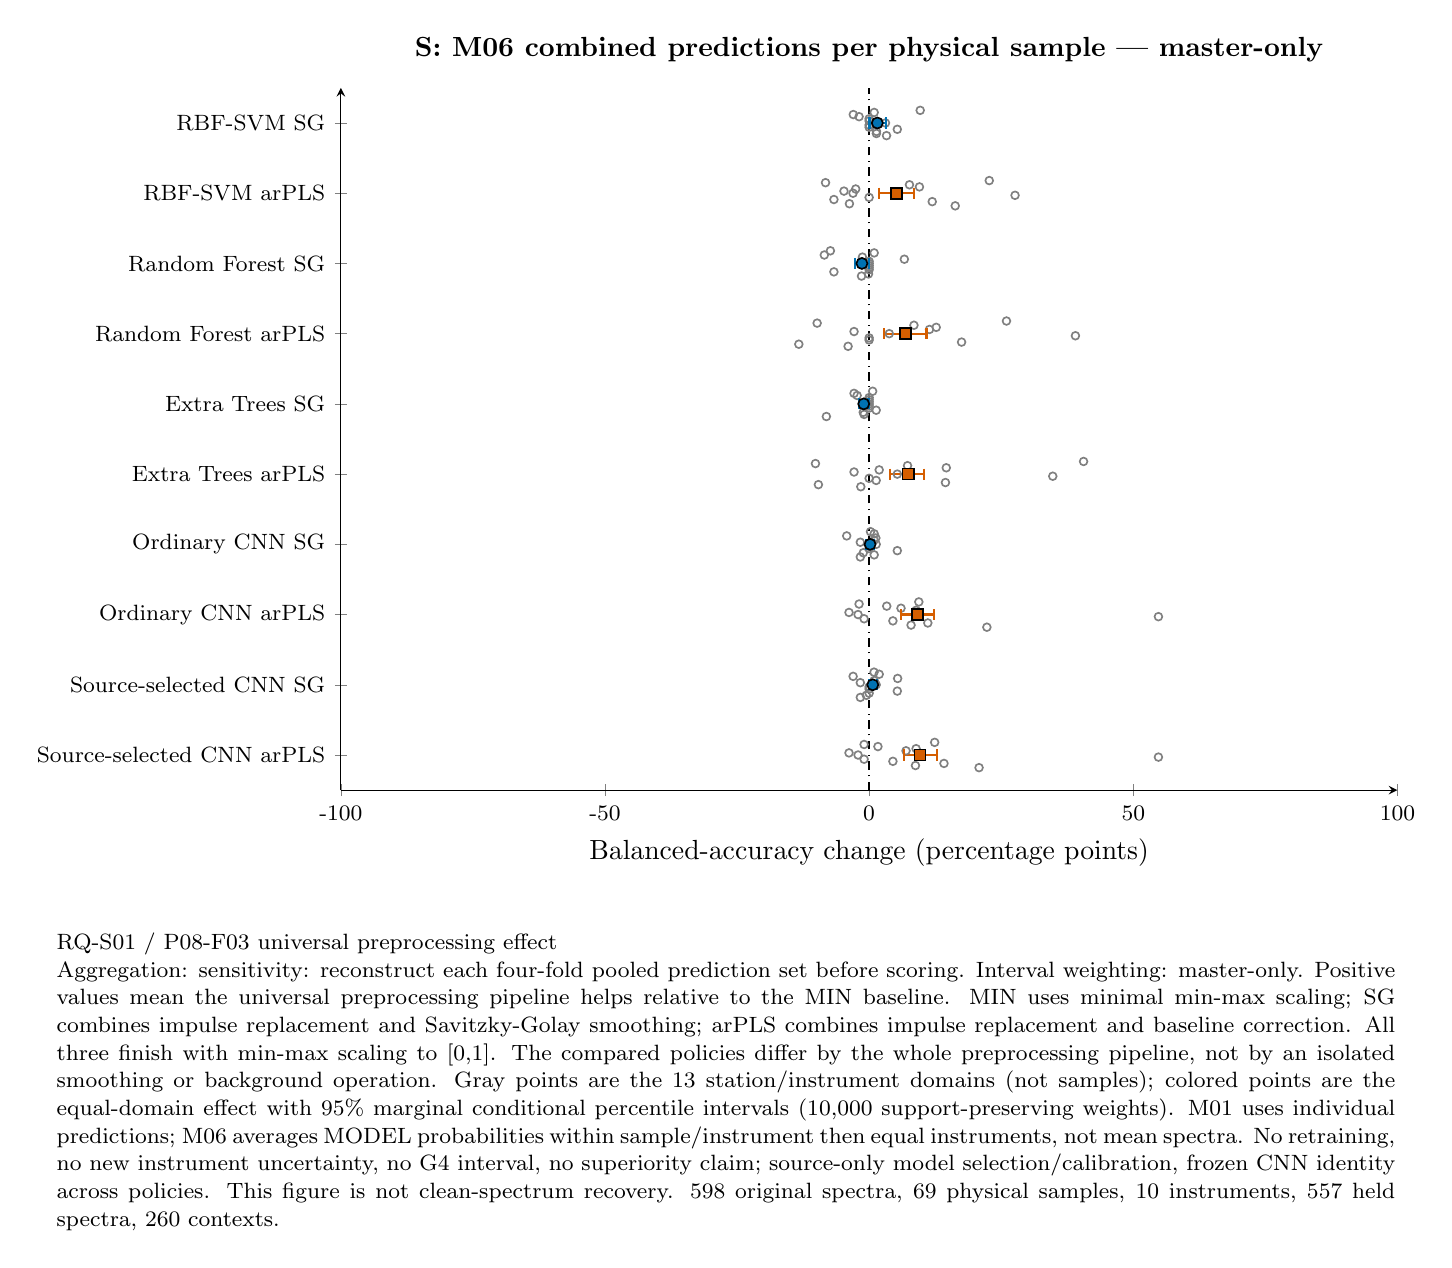
\begin{tikzpicture}
\begin{axis}[width=150mm, height=105mm, clip=false, xmin=-1, xmax=1, xtick={-1,-0.5,0,0.5,1}, xticklabels={-100,-50,0,50,100}, xlabel={Balanced-accuracy change (percentage points)}, ymin=-0.5, ymax=9.5, ytick={0,1,2,3,4,5,6,7,8,9}, yticklabels={{Source-selected CNN arPLS}, {Source-selected CNN SG}, {Ordinary CNN arPLS}, {Ordinary CNN SG}, {Extra Trees arPLS}, {Extra Trees SG}, {Random Forest arPLS}, {Random Forest SG}, {RBF-SVM arPLS}, {RBF-SVM SG}}, yticklabel style={font=\fontsize{8}{10}\selectfont}, tick label style={font=\fontsize{8}{10}\selectfont}, axis lines=left, title={S: M06 combined predictions per physical sample | master-only}, title style={font=\bfseries\fontsize{10}{12}\selectfont}, every axis plot/.append style={line width=0.6pt}]
\draw[black, dash dot, line width=0.6pt] (axis cs:0,-0.5) -- (axis cs:0,9.5);
\addplot[domainpts] coordinates {(0.032936507936507931,8.8200000000000003) (0.013756613756613753,8.8499999999999996) (0.013888888888888886,8.8800000000000008) (0.05333333333333333,8.9100000000000001) (0,8.9399999999999995) (0,8.9700000000000006) (0.03095238095238096,9) (0,9.0299999999999994) (0,9.0600000000000005) (-0.019047619047619046,9.0899999999999999) (-0.029999999999999999,9.1199999999999992) (0.0095238095238095229,9.1500000000000004) (0.096666666666666651,9.1799999999999997)};
\addplot[bar0] coordinates {(0.00059245532792668546,9) (0.032260789492213608,9)};
\addplot[pt0] coordinates {(0.015539275539275539,9)};
\addplot[domainpts] coordinates {(0.16296296296296298,7.8200000000000003) (-0.037301587301587301,7.8499999999999996) (0.11944444444444446,7.8799999999999999) (-0.066666666666666666,7.9100000000000001) (0,7.9400000000000004) (0.27619047619047621,7.9699999999999998) (-0.030476190476190473,8) (-0.047619047619047616,8.0299999999999994) (-0.0253968253968254,8.0600000000000005) (0.095238095238095219,8.0899999999999999) (0.07636363636363637,8.1199999999999992) (-0.082539682539682538,8.1500000000000004) (0.22740740740740742,8.1799999999999997)};
\addplot[bar1] coordinates {(0.018052717396840071,8) (0.084976794273083994,8)};
\addplot[pt1] coordinates {(0.051354386354386355,8)};
\addplot[domainpts] coordinates {(-0.014417989417989413,6.8200000000000003) (-0.0011904761904761904,6.8499999999999996) (-0.06666666666666668,6.8799999999999999) (0,6.9100000000000001) (0,6.9400000000000004) (0,6.9699999999999998) (0,7) (0,7.0300000000000002) (0.066666666666666666,7.0599999999999996) (-0.012698412698412698,7.0899999999999999) (-0.08484848484848484,7.1200000000000001) (0.0095238095238095229,7.1500000000000004) (-0.073333333333333334,7.1799999999999997)};
\addplot[bar0] coordinates {(-0.026142196208224392,7) (0.00021918420147156231,7)};
\addplot[pt0] coordinates {(-0.013612683612683613,7)};
\addplot[domainpts] coordinates {(-0.039814814814814817,5.8200000000000003) (-0.13306878306878306,5.8499999999999996) (0.17499999999999999,5.8799999999999999) (0,5.9100000000000001) (0,5.9400000000000004) (0.39047619047619042,5.9699999999999998) (0.038095238095238106,6) (-0.028571428571428571,6.0300000000000002) (0.11428571428571428,6.0599999999999996) (0.12698412698412698,6.0899999999999999) (0.08484848484848484,6.1200000000000001) (-0.098412698412698396,6.1500000000000004) (0.25999999999999995,6.1799999999999997)};
\addplot[bar1] coordinates {(0.028015811376910185,6) (0.10866905818524879,6)};
\addplot[pt1] coordinates {(0.068447848447848444,6)};
\addplot[domainpts] coordinates {(-0.080952380952380956,4.8200000000000003) (-0.0095238095238095229,4.8499999999999996) (-0.01111111111111111,4.8799999999999999) (0.013333333333333332,4.9100000000000001) (0,4.9400000000000004) (0,4.9699999999999998) (0,5) (0,5.0300000000000002) (0,5.0599999999999996) (0,5.0899999999999999) (-0.022727272727272728,5.1200000000000001) (-0.028571428571428571,5.1500000000000004) (0.0066666666666666662,5.1799999999999997)};
\addplot[bar0] coordinates {(-0.018857124782843935,5) (-0.0012679295516153986,5)};
\addplot[pt0] coordinates {(-0.010222000222000222,5)};
\addplot[domainpts] coordinates {(-0.015740740740740739,3.8199999999999998) (-0.096031746031746024,3.8500000000000001) (0.14444444444444443,3.8799999999999999) (0.013333333333333332,3.9100000000000001) (0,3.9399999999999999) (0.34761904761904761,3.9700000000000002) (0.05333333333333333,4) (-0.028571428571428571,4.0300000000000002) (0.019047619047619046,4.0599999999999996) (0.14603174603174601,4.0899999999999999) (0.072727272727272724,4.1200000000000001) (-0.10158730158730159,4.1500000000000004) (0.40592592592592591,4.1799999999999997)};
\addplot[bar1] coordinates {(0.039522133183160946,4) (0.10454010670877442,4)};
\addplot[pt1] coordinates {(0.073887038887038875,4)};
\addplot[domainpts] coordinates {(-0.016666666666666666,2.8199999999999998) (0.0095238095238095229,2.8500000000000001) (-0.01111111111111111,2.8799999999999999) (0.05333333333333333,2.9100000000000001) (0,2.9399999999999999) (0,2.9700000000000002) (0.013333333333333332,3) (-0.01666666666666667,3.0299999999999998) (0.0095238095238095229,3.0600000000000001) (0.012698412698412698,3.0899999999999999) (-0.042424242424242427,3.1200000000000001) (0.0095238095238095229,3.1499999999999999) (0.0025925925925925921,3.1800000000000002)};
\addplot[bar0] coordinates {(-0.0048298426935221416,3) (0.0086291856807483511,3)};
\addplot[pt0] coordinates {(0.0018200318200318191,3)};
\addplot[domainpts] coordinates {(0.22288359788359791,1.8200000000000001) (0.079365079365079347,1.8500000000000001) (0.11111111111111112,1.8799999999999999) (0.044999999999999998,1.9099999999999999) (-0.0095238095238095229,1.9399999999999999) (0.54761904761904767,1.97) (-0.020952380952380951,2) (-0.038095238095238092,2.0299999999999998) (0.088888888888888878,2.0600000000000001) (0.060317460317460311,2.0899999999999999) (0.03333333333333334,2.1200000000000001) (-0.019047619047619046,2.1499999999999999) (0.09407407407407406,2.1800000000000002)};
\addplot[bar1] coordinates {(0.061060559688537103,2) (0.12331136085224108,2)};
\addplot[pt1] coordinates {(0.091921041921041918,2)};
\addplot[domainpts] coordinates {(-0.016666666666666666,0.82000000000000006) (-0.0052910052910052907,0.84999999999999998) (0,0.88) (0.05333333333333333,0.91000000000000003) (0,0.93999999999999995) (0,0.96999999999999997) (0.013333333333333332,1) (-0.01666666666666667,1.03) (0.0095238095238095229,1.0600000000000001) (0.053968253968253964,1.0900000000000001) (-0.030303030303030304,1.1200000000000001) (0.019047619047619046,1.1499999999999999) (0.0092592592592592605,1.1799999999999999)};
\addplot[bar0] coordinates {(-0.00067570998155433947,1) (0.01488045654973958,1)};
\addplot[pt0] coordinates {(0.0068875568875568869,1)};
\addplot[domainpts] coordinates {(0.20806878306878307,-0.17999999999999999) (0.087698412698412692,-0.14999999999999999) (0.14166666666666666,-0.12) (0.044999999999999998,-0.089999999999999997) (-0.0095238095238095229,-0.059999999999999998) (0.54761904761904767,-0.029999999999999999) (-0.020952380952380951,0) (-0.038095238095238092,0.029999999999999999) (0.069841269841269843,0.059999999999999998) (0.088888888888888878,0.089999999999999997) (0.01666666666666667,0.12) (-0.0095238095238095229,0.14999999999999999) (0.12407407407407409,0.17999999999999999)};
\addplot[bar1] coordinates {(0.065388650451424599,0) (0.12790342208720903,0)};
\addplot[pt1] coordinates {(0.096263736263736271,0)};
\end{axis}
\node[anchor=north, align=justify, text width=170mm, font=\fontsize{8}{10}\selectfont] at ([yshift=-6mm]current bounding box.south) {RQ-S01 / P08-F03 universal preprocessing effect\\ Aggregation: sensitivity: reconstruct each four-fold pooled prediction set before scoring. Interval weighting: master-only. Positive values mean the universal preprocessing pipeline helps relative to the MIN baseline. MIN uses minimal min-max scaling; SG combines impulse replacement and Savitzky-Golay smoothing; arPLS combines impulse replacement and baseline correction. All three finish with min-max scaling to [0,1]. The compared policies differ by the whole preprocessing pipeline, not by an isolated smoothing or background operation. Gray points are the 13 station/instrument domains (not samples); colored points are the equal-domain effect with 95\% marginal conditional percentile intervals (10,000 support-preserving weights). M01 uses individual predictions; M06 averages MODEL probabilities within sample/instrument then equal instruments, not mean spectra. No retraining, no new instrument uncertainty, no G4 interval, no superiority claim; source-only model selection/calibration, frozen CNN identity across policies. This figure is not clean-spectrum recovery. 598 original spectra, 69 physical samples, 10 instruments, 557 held spectra, 260 contexts.};
\end{tikzpicture}
\end{minipage}
\end{document}
